\documentclass{beamer}
\usepackage{beamerthemesplit} % kam neu dazu
\usepackage[utf8]{inputenc}
\usepackage[T1]{fontenc}
\usepackage[ngerman]{babel}



\begin{document}
\title{Mößbauereffekt} 
\author{Paul Kremser, Tobias Grussenemyer}
\date{Versuchsdurchführung: 1. bis 12. März 2010} 

\frame{\titlepage} 

\frame{\frametitle{Inhaltsverzeichnis}\tableofcontents} 

\part{part1}

\section{Überblick}

\frame{\frametitle{Rudolf Mößbauer}
Er ging davon aus, dass sich zwei Quanten die auf diese Weise wechselwirken mit der doppelten Rückstoßgeschwindigkeit aufeinander zu bewegen müssten.
Diese Theorie folgt direkt aus der Impulserhaltung und schien zunächst auch durch das Experiment bestätigt zu werden. Zuerst untersuchte Mössbauer nämlich die
Resonanzabsorption bei Zimmertemperatur und darüber. Als er aber begann Quelle und Absorber abzukühlen, stieg die Intensität des Messsignals plötzlich steil an,
und zwar über die bei hohen Temperaturen gemessene.
}


\section{Aufgabenstellung}
\frame{\frametitle{Aufgabenstellung ??vielleicht rausnehmen??} 
\begin{enumerate}
 \item Verkabelung des Aufbaus, Einstellungen der Elektronik (Verstärker, Delay, SCA und Gate).
 \item Energieeichung des MCA mit Hilfe eines Americium Strahlers und verschiedener metallischer Floureszenzplättchen (Aufbau mit Drehscheibe)
 \item Mit dem SCA ein Fenster auf die 14,4 KeV Linie setzen.
 \item Mit Hilfe verschiedener Aluminiumplättchen sollen Untergrundmessungen bei verschiedenen Dicken gemacht werden um später auf die Dicke Null extrapolieren zu können.
 \item Aufnahme der Spektren des Einlinien- (Eisen) Absorbers und des 6-Linien- (Edelstahl) Absorbers.
\end{enumerate}
}

\section{Theoretische Grundlagen}
\subsection{Resonanzabsorption}
\frame{\frametitle{Resonanzabsorption}
\begin{itemize}[<+->]
 \item Beim Kernübergang von angeregtem- in Grundzustand
 \item wird ein Photon erzeugt $E_\gamma \approx E_a - E_g$
 \item dieses kann einen anderen Kern anregen
 \item Resonanzabsorption: Gleiche angeregte Zustände
 \item Aus der Impulserhaltung folgt ein Engergiefehlbetrag der doppelten Rückstoßenergie
\end{itemize}

\pause
 
\begin{figure}
 \includegraphics[width=0.9\linewidth]{pictures/linienskizze.ps}
 \caption{Energieverschiebung von Emissions- und Absorptionslinie}
 \label{linienskizze}
\end{figure}
}

\end{document}

